\documentclass[a4paper,oneside,12pt]{report}
% Package yang diperlukan
\usepackage{fontspec}       % Font sistem untuk XeLaTeX/LuaLaTeX
\usepackage{amsmath}        % Simbol dan format matematika
\usepackage{setspace}       % Pengaturan jarak antarbaris
\usepackage{graphicx}      % Untuk memasukkan gambar
\usepackage{titling}       % Untuk kustomisasi halaman judul
\usepackage{geometry}      % Untuk mengatur margin halaman
\usepackage{listings}      % Untuk menampilkan blok kode
\usepackage{xcolor}        % Untuk menggunakan warna
\usepackage{float}         % Untuk kontrol penempatan float (seperti gambar)
\usepackage{hyperref}      % Untuk membuat hyperlink (URL, referensi)
\usepackage{indentfirst}   % Untuk memberi indentasi pada paragraf pertama setiap seksi
\usepackage{url}           % Untuk format URL
\usepackage{xurl}          % Untuk pemotongan URL panjang agar rapi
\usepackage{fancyhdr}      % Untuk kustomisasi header dan footer
\usepackage{tocloft}       % Untuk kustomisasi Daftar Isi
\usepackage{bookmark}      % Untuk manajemen bookmark PDF yang lebih baik

% Font dan spasi standar laporan praktikum
\setmainfont{TeX Gyre Termes}
\onehalfspacing

%======================================================================
% PENGATURAN GEOMETRI HALAMAN DAN JUSTIFIKASI TEKS
%======================================================================
\geometry{left=3cm, right=2.5cm, top=2cm, bottom=2.5cm}
\sloppy
\tolerance=9999
\emergencystretch=3em
\hyphenpenalty=10000
\exhyphenpenalty=10000

%======================================================================
% PENGATURAN WARNA UNTUK BLOK KODE
%======================================================================
\definecolor{codegreen}{rgb}{0,0.6,0}
\definecolor{codegray}{rgb}{0.5,0.5,0.5}
\definecolor{codepurple}{rgb}{0.58,0,0.82}
\definecolor{backcolour}{rgb}{0.95,0.95,0.92}
\definecolor{darkblue}{rgb}{0,0,0.6}

%======================================================================
% PENGATURAN BLOK KODE (LISTINGS)
%======================================================================
\lstdefinestyle{commonstyle}{
    backgroundcolor=\color{backcolour},
    breakatwhitespace=false,
    breaklines=true,
    captionpos=b,
    keepspaces=true,
    numbers=left,
    numbersep=5pt,
    showspaces=false,
    showstringspaces=false,
    showtabs=false,
    tabsize=2,
    frame=single,
    basicstyle=\ttfamily\footnotesize,
    numberstyle=\tiny\color{codegray},
    columns=flexible,
    postbreak=\mbox{\textcolor{red}{$\hookrightarrow$}\space},
    breakindent=0pt,
    breakautoindent=false
}

%======================================================================
% PENGATURAN LAIN-LAIN
%======================================================================
\newcommand{\customfbox}[1]{%
  \setlength{\fboxsep}{0pt}%
  \setlength{\fboxrule}{0.5pt}%
  \fcolorbox{black}{white}{#1}%
}
\renewcommand{\figurename}{Gambar}
\renewcommand{\thefigure}{\arabic{figure}}
\hypersetup{
    colorlinks=true,
    linkcolor=black,
    filecolor=black,
    urlcolor=black,
    citecolor=black,
    pdftitle={Laporan Praktikum PPG Pertemuan 6},
    pdfpagemode=UseOutlines,
    breaklinks=true
}
\pagestyle{fancy}
\fancyhf{}
\fancyfoot[C]{\thepage}
\renewcommand{\headrulewidth}{0pt}
\fancypagestyle{plain}{
    \fancyhf{}
    \fancyfoot[C]{\thepage}
    \renewcommand{\headrulewidth}{0pt}
}
\renewcommand{\contentsname}{Daftar Isi}
\renewcommand{\bibname}{Daftar Pustaka}
\renewcommand{\thechapter}{}
\renewcommand{\chaptername}{}
\renewcommand{\thesection}{\arabic{chapter}.\arabic{section}}
\renewcommand{\thesubsection}{\thesection.\arabic{subsection}}
\setcounter{secnumdepth}{3}
\setcounter{tocdepth}{3}
\renewcommand{\cftchapdotsep}{\cftdotsep}
\renewcommand{\cftchapleader}{\cftdotfill{\cftchapdotsep}}
\setlength{\cftchapindent}{0em}
\setlength{\cftsecindent}{2em}
\setlength{\cftsubsecindent}{4em}
\setlength{\cftchapnumwidth}{0em}
\setlength{\cftsecnumwidth}{2.5em}
\setlength{\cftsubsecnumwidth}{3.2em}
\renewcommand{\cftchappresnum}{}
\renewcommand{\cftchapaftersnum}{}
\newcommand{\tocboldsection}[1]{%
  \protect\renewcommand{\protect\cftchapfont}{\protect\bfseries}%
  #1%
  \protect\renewcommand{\protect\cftchapfont}{}%
}
\pdfstringdefDisableCommands{\def\tocboldsection#1{#1}}

%======================================================================
% AWAL DOKUMEN
%======================================================================
\begin{document}

% Halaman Judul
\newgeometry{left=3cm, right=2.5cm, top=2.5cm, bottom=3cm}
\begin{titlingpage}
	\begin{spacing}{1}
		\begin{center}
			\vspace*{0.2cm}
			{\large \textbf{\MakeUppercase{Laporan Praktikum}}} \\[0.4cm]
			{\large \textbf{\MakeUppercase{PRAKTIKUM PENGEMBANGAN GAME}}} \\[0.4cm]
			{\large \textbf{\MakeUppercase{Pertemuan 6}}} \\[0.4cm]
			{\large \textbf{\MakeUppercase{LANDSCAPE, RIG, RETARGET, DAN ANIMATION}}} \\[1.5cm]

			
\includegraphics[height=7cm]{images/UGM.png} \\[0.7cm]

			{\normalsize \textbf{Disusun oleh:}} \\[0.4cm]
			\begin{tabular}{@{}l l @{}}
				\textbf{Nama}           & : Hafidz Rizqullah Prasetya                   \\
				\textbf{NIM}            & : 24/535493/SV/24243                          \\
				\textbf{NIU}            & : 535493                                      \\
				\textbf{Kelas}          & : PL5A1                                       \\
				\textbf{Dosen Pengampu} & : Yusron Fuadi, S.Sn., M.Sn.                  \\
				\textbf{Asisten}        & : Ezra Bariq Rizqullah / Ikhwan Hanif Firdaus \\
			\end{tabular} \\[1.2cm]

			{\normalsize \textbf{PROGRAM STUDI D-IV}} \\[0.2cm]
			{\normalsize \textbf{TEKNOLOGI REKAYASA PERANGKAT LUNAK}} \\[0.2cm]
			{\normalsize \textbf{DEPARTEMEN TEKNIK ELEKTRO DAN INFORMATIKA}} \\[0.2cm]
			{\normalsize \textbf{SEKOLAH VOKASI}} \\[0.2cm]
			{\normalsize \textbf{UNIVERSITAS GADJAH MADA}} \\[0.2cm]
			{\normalsize \textbf{YOGYAKARTA}} \\[0.2cm]
			{\normalsize \textbf{2026}} \\[1.2cm]
		\end{center}
	\end{spacing}
\end{titlingpage}
\restoregeometry

\thispagestyle{empty}
\clearpage
\stepcounter{page}
\thispagestyle{empty}

% --- Daftar Isi ---
\addcontentsline{toc}{chapter}{Daftar Isi}
\tableofcontents
\clearpage

% Mengatur penomoran halaman menjadi arab dan mulai dari 3
\pagenumbering{arabic}
\setcounter{page}{3}

\chapter[Tujuan Praktikum]{Tujuan Praktikum}
\begin{enumerate}
	\item Mahasiswa memahami struktur berkas level berekstensi \texttt{.umap} dalam Unreal Engine 5.8 serta pertimbangan teknis pemilihan \textit{Empty Level} dibanding \textit{World Partition} pada pengembangan prototipe game \cite{modul6,epic-levels}.
	\item Mahasiswa mampu mengonfigurasi sistem tata cahaya dan atmosfer level menggunakan \textit{Environment Light Mixer} secara terpadu \cite{modul6,epic-lightmixer}.
	\item Mahasiswa mampu merancang dan memanipulasi bentang alam (\textit{landscape}) melalui teknik pembentukan kontur (\textit{sculpting}) serta pengaplikasian material permukaan dasar \cite{modul6,epic-landscape,epic-sculpt}.
	\item Mahasiswa memahami perbedaan struktur kerangka (\textit{rigging}) antara karakter Mixamo berbasis T-Pose dan Unreal Engine Mannequin berbasis A-Pose, serta mampu menerapkan alur kerja \textit{IK Retargeting} untuk mentransfer animasi \cite{modul6,epic-skeletal,epic-retargeter,mixamo-web}.
	\item Mahasiswa mampu membuat dan mengintegrasikan \textit{Animation Montage} ke dalam sistem kendali karakter melalui \textit{Animation Blueprint} dan masukan tombol keyboard pada \textit{Event Graph} \cite{modul6,epic-montage,epic-naming}.
\end{enumerate}
\clearpage

\chapter{Dasar Teori}

\section{Arsitektur Level dan Bentang Alam pada Unreal Engine}
Level merupakan ruang virtual tempat seluruh aktor, sistem pencahayaan, geometri lingkungan, dan logika permainan ditempatkan \cite{epic-levels}. Pada Unreal Engine, level disimpan ke dalam berkas berekstensi \texttt{.umap}. Dalam pengembangan proyek, pemilihan template level menentukan sistem pengelolaan memori dunia. Unreal Engine 5 menyediakan sistem \textit{World Partition} untuk memecah dunia berskala besar menjadi petak-petak kecil yang dimuat secara dinamis saat runtime \cite{epic-levels}.

Pada prototipe berskala kecil, sistem World Partition cenderung menambah kerumitan alur kerja karena menghasilkan entitas berupa \textit{Instanced Landscape}. Objek bentang alam instansiasi ini memiliki penanganan material dan partisi data yang berbeda dibanding bentang alam standar. Penggunaan \textit{Empty Level} menghasilkan objek \texttt{Landscape} murni, sehingga pengelolaan data elevasi dan material tetap stabil dan mudah diprediksi untuk kebutuhan praktikum \cite{modul6}.

Sistem bentang alam Unreal Engine dibangun menggunakan hierarki quad, section, dan komponen \cite{epic-landscape}. Satuan dasar permukaan dibentuk oleh quad, yaitu persegi terkecil yang terdiri dari dua poligon segitiga. Kumpulan quad membentuk satu section, dan gabungan section menyusun satu komponen landscape. Parameter \textit{Section Size} menentukan kerapatan titik verteks yang dapat dimanipulasi saat proses pembentukan kontur tanah. Pemilihan ukuran 15x15 quads memberikan pembagian grid yang efisien untuk area berukuran sedang dengan beban perhitungan rendering yang ringan \cite{epic-landscape}.

\section{Pencahayaan Lingkungan Menggunakan Environment Light Mixer}
Ruang kosong pada level baru tidak memiliki pencahayaan bawaan, sehingga tampilan viewport tampak hitam pekat. Penataan tata cahaya realistis membutuhkan integrasi beberapa aktor pencahayaan fisik yang saling melengkapi \cite{epic-lightmixer}. Unreal Engine menyediakan jendela \textit{Environment Light Mixer} untuk mengonfigurasi lima komponen lingkungan utama secara serempak:
\begin{enumerate}
	\item \textbf{Directional Light}: Mensimulasikan sumber cahaya berjarak tak terhingga, seperti matahari atau bulan, yang memancarkan berkas sinar sejajar ke seluruh level \cite{epic-lightmixer}.
	\item \textbf{Sky Light}: Menangkap informasi warna dari kubah langit dan memancarkannya kembali ke permukaan objek sebagai pencahayaan difus (\textit{ambient light}) \cite{epic-lightmixer}.
	\item \textbf{Sky Atmosphere}: Menghitung hamburan cahaya berbasis hukum fisika Rayleigh dan Mie di lapisan udara, menghasilkan gradasi warna langit yang realistis sesuai sudut datang cahaya matahari \cite{epic-lightmixer}.
	\item \textbf{Volumetric Cloud}: Menyusun partikel awan tiga dimensi melalui teknik komputasi \textit{ray marching}, memungkinkan awan menerima bayangan dari matahari secara dinamis \cite{epic-lightmixer}.
	\item \textbf{Exponential Height Fog}: Menghasilkan kabut berbasis kerapatan eksponensial terhadap ketinggian sumbu Z, memberikan petunjuk persepsi kedalaman ruang pada area terbuka \cite{epic-lightmixer}.
\end{enumerate}

Pengaturan kelima komponen ini melalui jendela terpadu memangkas waktu penyiapan lingkungan dasar tanpa perlu menambahkan aktor satu demi satu dari panel penempatan \cite{modul6}.

\section{Konsep Rigging dan Perbandingan Struktur Kerangka}
Model tiga dimensi visual pada dasarnya berupa susunan titik koordinat, garis rusuk, dan permukaan poligon yang kaku (\textit{Static Mesh}). Supaya model tersebut dapat digerakkan, diperlukan struktur kerangka tulang digital melalui proses yang disebut \textit{rigging} \cite{epic-skeletal}. Model yang telah dihubungkan dengan kerangka dinamakan \textit{Skeletal Mesh}. Setiap titik verteks pada jala model dikaitkan ke satu atau beberapa tulang dengan bobot pengaruh tertentu (\textit{skinning weight}) bernilai antara 0 hingga 1. Ketika sebuah sendi tulang berotasi, permukaan jala di sekitarnya akan terdeformasi mengikuti pergerakan tersebut \cite{epic-skeletal}.

Dalam industri game dan animasi, terdapat beragam standar struktur kerangka. Platform Adobe Mixamo menyediakan pustaka model dan animasi siap pakai yang menggunakan pose dasar \textit{T-Pose}, di mana kedua lengan karakter merentang lurus horizontal \cite{mixamo-web}. Sementara itu, karakter referensi Unreal Engine 5, yaitu Manny dan Quinn, menggunakan pose dasar \textit{A-Pose}, di mana kedua lengan mengarah serong ke bawah membentuk sudut sekitar 45 derajat \cite{epic-skeletal}. Perbedaan pose dasar, orientasi sumbu lokal tulang, serta penamaan hierarki sendi menyebabkan animasi yang direkam untuk kerangka Mixamo tidak dapat diputar langsung pada kerangka Unreal Engine tanpa penyesuaian awal \cite{modul6}.

Kerangka Mixamo tidak memiliki rig wajah (\textit{facial rig}) terperinci, sehingga model hanya mendukung artikulasi tubuh utama \cite{mixamo-web}. Pada tingkatan produksi fidelitas tinggi, teknologi seperti MetaHuman menyediakan struktur rig wajah parametrik yang kompleks untuk kebutuhan animasi ekspresi mikro dan sinkronisasi bibir \cite{epic-metahuman}. Namun untuk kebutuhan prototipe mekanik gerak, rig Mixamo memberikan efisiensi yang memadai.

\section{Mekanisme IK Retargeting dan Evaluasi Animasi}
Retargeting merupakan teknik komputasi grafika untuk memindahkan data pergerakan animasi dari satu kerangka sumber (\textit{source skeleton}) ke kerangka target (\textit{target skeleton}) yang memiliki proporsi ukuran atau hierarki berbeda \cite{epic-retargeter}. Unreal Engine 5 memanfaatkan sistem \textit{IK Rig} dan \textit{IK Retargeter} untuk memetakan rantai kinematika terbalik (\textit{Inverse Kinematics chains}), seperti rantai tulang lengan, kaki, dan tulang belakang \cite{epic-retargeter}.

\begin{equation}
	\mathbf{P}_{\text{target}}(t) = f_{\text{retarget}}(\mathbf{P}_{\text{source}}(t), \mathbf{Pose}_{\text{source\_ref}}, \mathbf{Pose}_{\text{target\_ref}})
\end{equation}

Persamaan di atas menggambarkan pemetaan transformasi tulang target $\mathbf{P}_{\text{target}}(t)$ pada waktu $t$ yang dipengaruhi oleh perbedaan pose referensi awal antara kedua model. Dengan menyelaraskan pose awal melalui rotasi tulang lengan atas karakter Mixamo agar menyerupai A-Pose milik Mannequin, data rotasi dan translasi dapat ditransfer secara akurat tanpa distorsi visual pada sambungan sendi bahu \cite{epic-retargeter}.

Pada implementasi runtime, Unreal Engine menyediakan node \texttt{Retarget Pose From Mesh} di dalam \textit{AnimGraph} milik \textit{Animation Blueprint} \cite{modul6}. Node ini membaca pose gerak dari mesh utama secara langsung dan menerapkan hasil pemetaan ke skeletal mesh target pada setiap frame. Agar proses pembacaan pose tetap berjalan ketika mesh utama disembunyikan dari layar, properti \textit{Visibility Based Anim Tick Option} pada komponen skeletal mesh harus disetel ke opsi \textit{Always Tick Pose and Refresh Bones} \cite{modul6}. Pengaturan ini memastikan mesin terus menghitung transformasi tulang di latar belakang, sehingga karakter kustom target tidak mengalami pembekuan pose gerak \cite{modul6}.

\section{Modularitas Gerak Melalui Animation Montage}
Aset \textit{Animation Sequence} menyimpan rekaman pergerakan tulang berbasis waktu untuk aksi tertentu, seperti berjalan atau berlari \cite{epic-skeletal}. Jika animasi aksi sesaat, seperti tarian atau serangan, diputar langsung menggantikan state machine utama, alur logika perpindahan pose dasar akan terputus. Unreal Engine menyediakan \textit{Animation Montage} sebagai lapisan pengendali gerak yang fleksibel \cite{epic-montage}.

Animation Montage membungkus animation sequence ke dalam struktur yang dapat dibagi menjadi beberapa segmen (\textit{sections}) dan slot pembauran (\textit{slots}) \cite{epic-montage}. Melalui pemanfaatan node \texttt{Slot 'DefaultSlot'} pada AnimGraph, sebuah montage dapat dipicu secara programatik melalui Blueprint menggunakan node \texttt{Play Anim Montage}. Sistem ini menerapkan parameter waktu \textit{Blend In} dan \textit{Blend Out} agar transisi dari gerakan berjalan ke gerakan montage berlangsung halus tanpa patahan pose yang kaku \cite{epic-montage}.

\clearpage

\chapter[\tocboldsection{Hasil dan Pembahasan}]{Hasil dan Pembahasan}

Praktikum Pertemuan 6 dilaksanakan pada proyek Unreal Engine 5.8 \texttt{HAFIDZ\_535493\_PPG}. Proyek ini merupakan kelanjutan langsung dari sesi praktikum sebelumnya, memanfaatkan template dasar Third Person yang telah memuat struktur folder karakter, peta, serta logika pemain. Seluruh langkah praktikum didokumentasikan secara berurutan sesuai alur modul pembelajaran, mencakup penataan lingkungan bentang alam, integrasi karakter Mixamo, hingga pengujian animasi montage.

\section{Dokumentasi Praktikum}

\subsection{Pembuatan Level Baru dan Penataan Tata Cahaya}

\begin{enumerate}
	\item \textbf{Pembuatan Empty Level (LV\_Praktikum).} Melalui menu \textbf{File > New Level} atau kombinasi tombol \texttt{Ctrl + N}, jendela pemilihan tipe level dibuka. Pilihan diarahkan ke opsi \textbf{Empty Level} untuk menghindari pembuatan partisi dunia otomatis (\textit{World Partition}). Berkas level baru ini kemudian disimpan ke dalam folder proyek dengan nama \textbf{LV\_Praktikum}. Penggunaan level kosong menjamin stabilitas objek bentang alam tunggal tanpa komplikasi instansiasi partisi.

	      \begin{figure}[H]
		      \centering
		      \customfbox{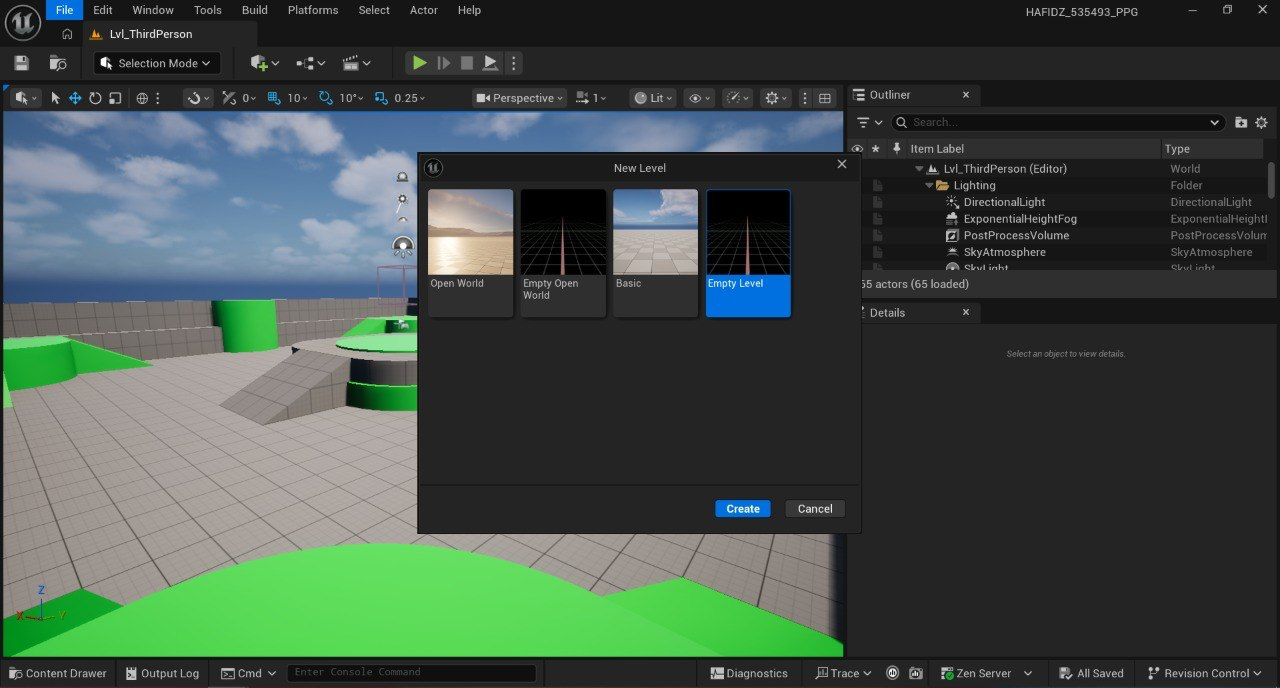
\includegraphics[width=0.9\textwidth]{images/ss-01-new-level-empty.png}}
		      \caption{Pembuatan Empty Level baru dan penyimpanannya sebagai LV\_Praktikum pada Content Drawer.}
		      \label{fig:ss-new-level-empty}
	      \end{figure}

	      Pada Gambar \ref{fig:ss-new-level-empty}, jendela pembuatan level menampilkan tiga opsi utama: Open World, Basic, dan Empty Level. Opsi Empty Level dipilih karena kebutuhan praktikum berfokus pada area terbatas yang tidak memerlukan pemuatan sel partisi latar belakang. Level yang berhasil dibuat disimpan dengan ekstensi \texttt{.umap} pada folder Content Drawer, siap untuk diisi komponen lingkungan.

	\item \textbf{Konfigurasi Tata Cahaya Lingkungan.} Kondisi awal level yang gelap pekat diatasi dengan membuka jendela \textbf{Window > Env. Light Mixer}. Pada jendela ini, tombol pembuatan diklik untuk kelima komponen pencahayaan lingkungan fisik: \textit{Directional Light}, \textit{Sky Light}, \textit{Sky Atmosphere}, \textit{Volumetric Cloud}, dan \textit{Exponential Height Fog}.

	      \begin{figure}[H]
		      \centering
		      \customfbox{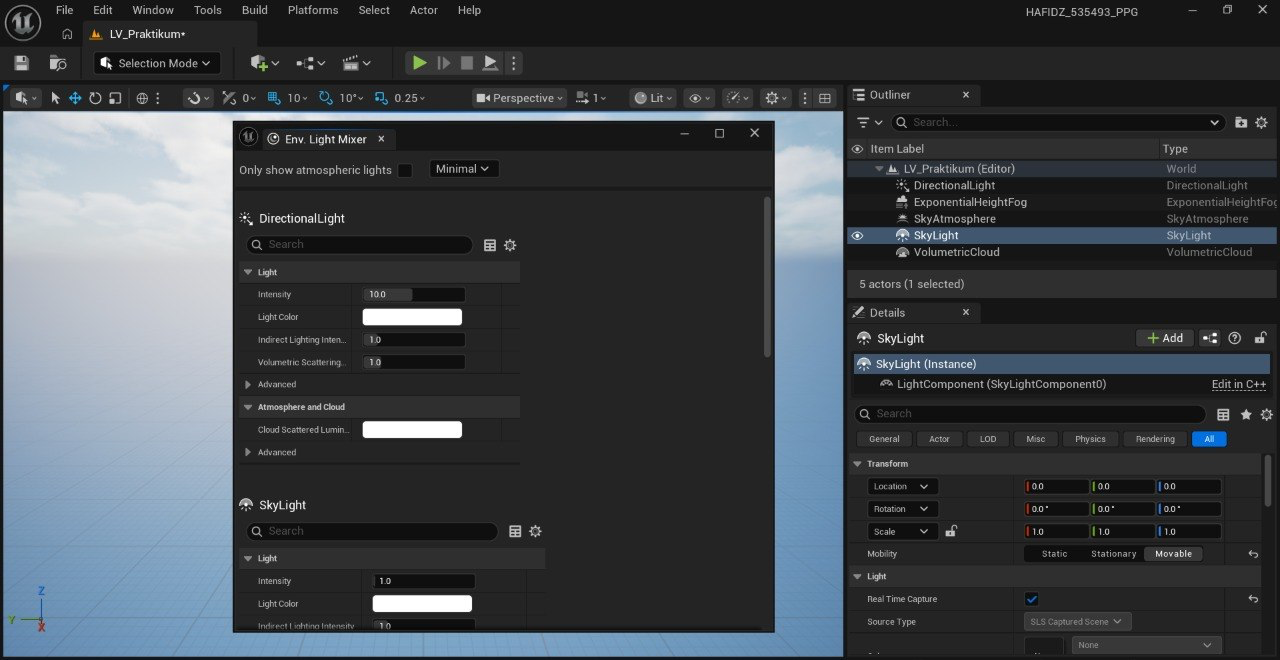
\includegraphics[width=0.9\textwidth]{images/ss-02-env-light-mixer.png}}
		      \caption{Aktivasi kelima komponen pencahayaan lingkungan melalui Environment Light Mixer.}
		      \label{fig:ss-env-light-mixer}
	      \end{figure}

	      Gambar \ref{fig:ss-env-light-mixer} menunjukkan antarmuka Environment Light Mixer setelah kelima tombol create ditekan. Sinar matahari langsung dihasilkan oleh Directional Light, sementara kubah langit dan hamburan atmosfer dimodelkan secara serempak oleh Sky Atmosphere. Visual awan tiga dimensi dan persepsi kabut kedalaman langsung aktif di viewport tanpa perlu menyetel koordinat aktor secara manual.

\end{enumerate}

\subsection{Pembuatan dan Pembentukan Kontur Bentang Alam}

\begin{enumerate}
	\item \textbf{Pembuatan Grid Landscape Baru.} Mode kerja editor dialihkan ke \textbf{Landscape Mode} melalui toolbar atas atau menekan shortcut \texttt{Shift + 2}. Pada panel konfigurasi \textit{Manage / New Landscape}, parameter \textbf{Section Size} diubah nilainya menjadi \textbf{15x15 Quads}, sedangkan parameter lainnya dipertahankan pada nilai baku mesin. Tombol \textbf{Create} ditekan untuk menghasilkan bidang tanah datar baru.

	      \begin{figure}[H]
		      \centering
		      \customfbox{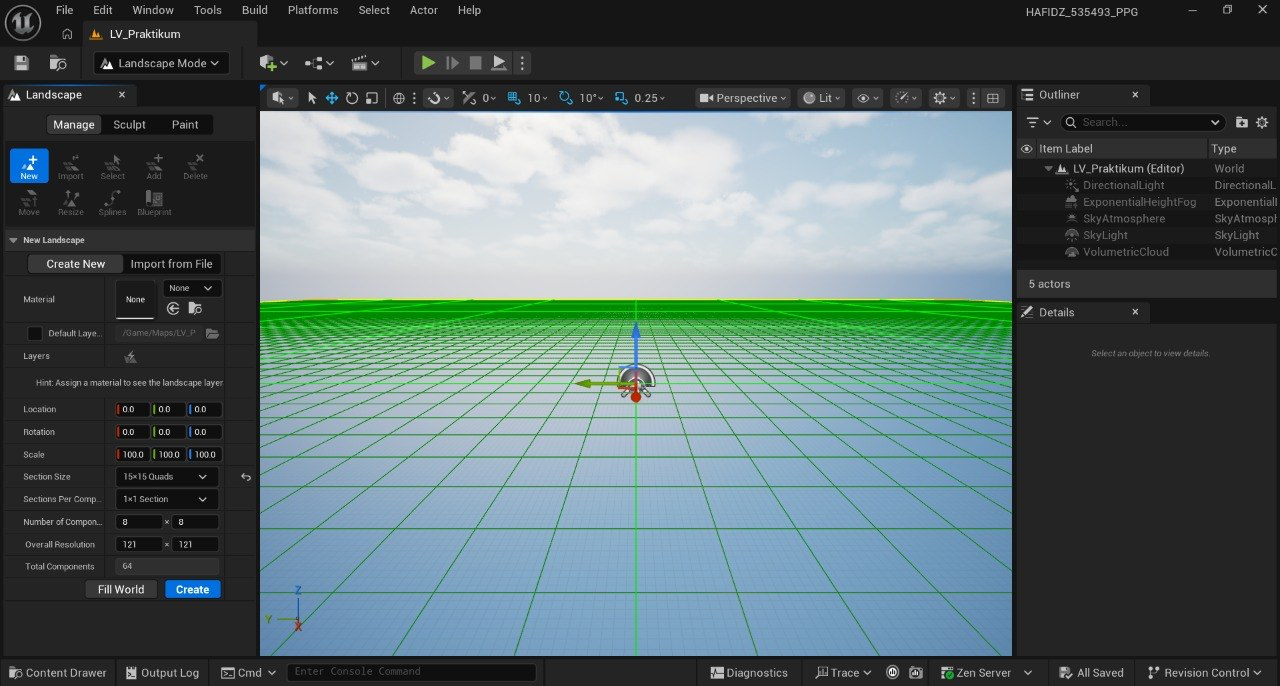
\includegraphics[width=0.9\textwidth]{images/ss-03-create-landscape.png}}
		      \caption{Pengaturan parameter Section Size 15x15 Quads pada panel pembentukan Landscape baru.}
		      \label{fig:ss-create-landscape}
	      \end{figure}

	      Gambar \ref{fig:ss-create-landscape} memperlihatkan grid hijau kawat yang menjadi panduan dimensi bentang alam sebelum digenerasi. Penyetelan ukuran section ke 15x15 quads menghasilkan kerapatan simpul yang pas untuk skala uji coba karakter. Struktur grid ini membagi beban perhitungan elevasi tanah secara seimbang sehingga proses editing tetap responsif.

	\item \textbf{Pembentukan Elevasi Kontur (Sculpting).} Setelah grid tanah terpasang, permukaan tanah dimanipulasi menggunakan kuas pemahat (\textit{sculpt tools}). Kuas \textbf{Sculpt} digunakan untuk menaikkan elevasi bukit, kuas \textbf{Smooth} diaplikasikan untuk meratakan sudut-sudut tajam yang bergerigi, serta alat bantu \textbf{Flatten} dan \textbf{Ramp} dimanfaatkan untuk membuat area datar dan tanjakan landai.

	      \begin{figure}[H]
		      \centering
		      \customfbox{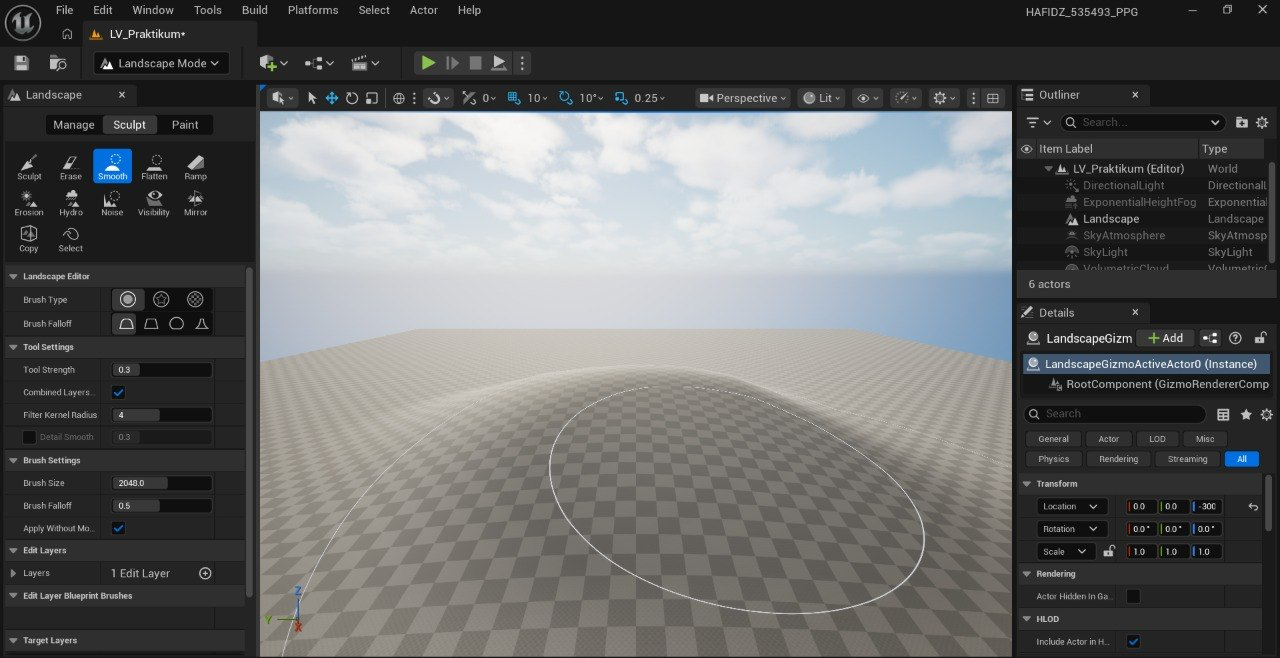
\includegraphics[width=0.9\textwidth]{images/ss-04-sculpting-landscape.png}}
		      \caption{Manipulasi permukaan tanah menggunakan variasi kuas Sculpt dan Smooth pada Landscape Mode.}
		      \label{fig:ss-sculpting-landscape}
	      \end{figure}

	      Pada Gambar \ref{fig:ss-sculpting-landscape}, kontur permukaan tanah di sekitar area awal pemain tampak memiliki variasi ketinggian bergelombang. Manipulasi elevasi ini memberikan rintangan topografi alami yang berguna untuk menguji interaksi pijakan kaki karakter serta kestabilan pergerakan kamera permainan.

	\item \textbf{Penerapan Material Permukaan Tanah.} Mode kerja dikembalikan ke \textbf{Selection Mode} (\texttt{Shift + 1}). Objek Landscape dipilih pada viewport, kemudian pada panel \textit{Details}, bagian properti \textbf{Landscape Material} dicari. Slot material tersebut diisi dengan material bawaan engine \textbf{CausticsBaseMesh} untuk memberikan visual pola permukaan bertekstur.

	      \begin{figure}[H]
		      \centering
		      \customfbox{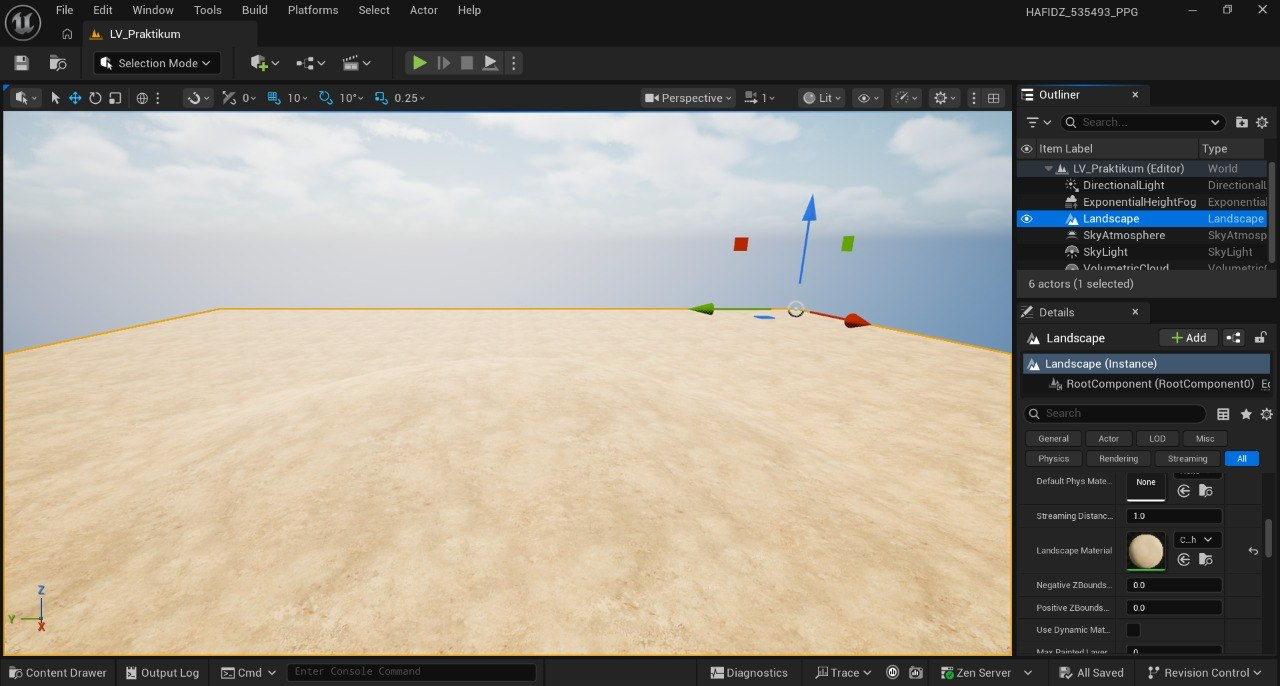
\includegraphics[width=0.9\textwidth]{images/ss-05-landscape-material.png}}
		      \caption{Pemasangan material CausticsBaseMesh pada slot Landscape Material objek Landscape.}
		      \label{fig:ss-landscape-material}
	      \end{figure}

	      Gambar \ref{fig:ss-landscape-material} menampilkan panel Details sisi kanan dengan kolom Landscape Material yang terisi aset CausticsBaseMesh. Permukaan bentang alam yang sebelumnya hanya berupa pola kotak-kotak abu-abu kini menampilkan refleksi pencahayaan material dasar, menegaskan bentuk lekukan tanah yang telah dipahat.

\end{enumerate}

\subsection{Impor dan Penataan Aset Karakter Kustom Mixamo}

\begin{enumerate}
	\item \textbf{Pengunduhan Karakter dan Animasi dari Mixamo.} Melalui peramban web, situs \texttt{mixamo.com} diakses. Sesuai panduan modul, navigasi dilakukan berurutan: memilih karakter pada tab \textbf{Characters} (misalnya karakter bernama Mousey), kemudian memilih animasi aksi pada tab \textbf{Animations}. Tombol \textbf{Download} ditekan dengan konfigurasi format \textbf{FBX Binary (.fbx)}, opsi Skin \textbf{With Skin}, dan laju bingkai 30 atau 60 FPS.

	      \begin{figure}[H]
		      \centering
		      \customfbox{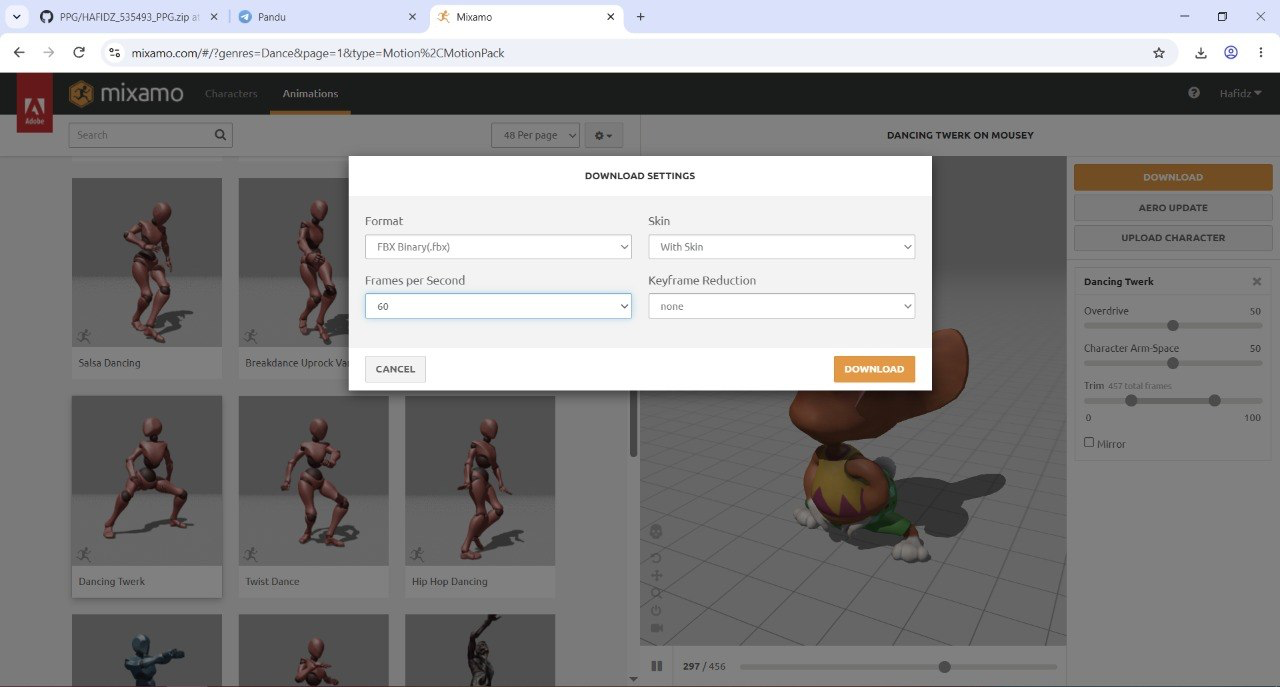
\includegraphics[width=0.9\textwidth]{images/ss-06-mixamo-download.png}}
		      \caption{Antarmuka pengunduhan aset karakter Mousey dan animasi aksi pada situs Mixamo.}
		      \label{fig:ss-mixamo-download}
	      \end{figure}

	      Pada Gambar \ref{fig:ss-mixamo-download}, jendela dialog Download Settings menampilkan pilihan FBX Binary dengan opsi With Skin. Memilih karakter terlebih dahulu sebelum animasi memastikan struktur proporsi kerangka tulang pada berkas animasi terikat secara tepat dengan jala model karakter yang diunduh.

	\item \textbf{Impor Berkas FBX ke Direktori Proyek.} Di dalam Content Drawer, direktori \texttt{Content/Characters} dibuka dan dibuatkan subfolder baru bernama \textbf{Mixamo}. Berkas FBX hasil unduhan ditarik masuk (\textit{drag and drop}) ke dalam folder tersebut. Pada jendela dialog \textbf{FBX Import Options}, tombol \textbf{Use Pipeline Defaults} diklik untuk mereset seluruh opsi impor ke nilai standar, lalu tombol \textbf{Import} ditekan.

	      \begin{figure}[H]
		      \centering
		      \customfbox{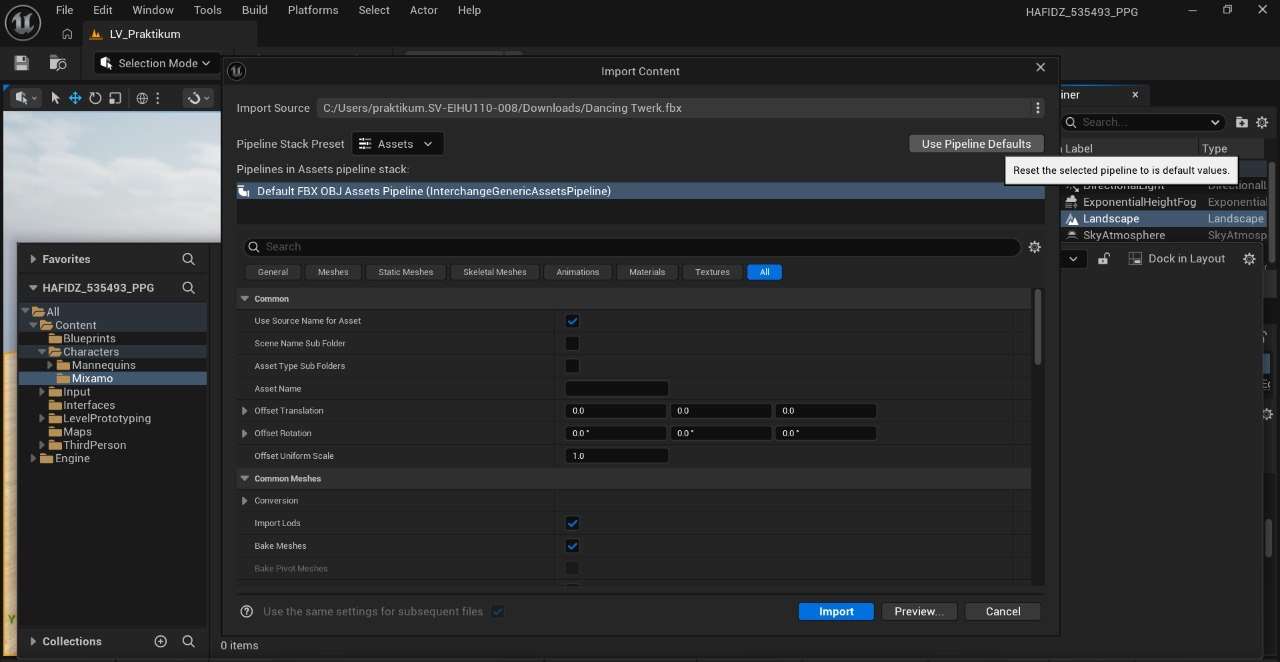
\includegraphics[width=0.9\textwidth]{images/ss-07-import-fbx-mixamo.png}}
		      \caption{Jendela FBX Import Options saat mengimpor model karakter kustom ke folder Mixamo.}
		      \label{fig:ss-import-fbx-mixamo}
	      \end{figure}

	      Gambar \ref{fig:ss-import-fbx-mixamo} menunjukkan proses impor FBX di mana mesin secara otomatis mendeteksi keberadaan skeletal mesh, material, dan struktur tulang. Penggunaan opsi pipeline default mencegah terjadinya kesalahan orientasi sumbu model saat diekstrak ke dalam format biner Unreal Engine.

	\item \textbf{Penyeragaman Konvensi Penamaan Aset.} Setelah proses impor selesai, sejumlah aset terbentuk di dalam folder Mixamo. Nama masing-masing aset diubah agar mematuhi standar penamaan resmi Epic Games: \textbf{SKM\_Mousey} untuk Skeletal Mesh, \textbf{SK\_Mousey} untuk Skeleton, \textbf{PHYS\_Mousey} untuk Physics Asset, serta \textbf{AS\_Emote} untuk Animation Sequence.

	      \begin{figure}[H]
		      \centering
		      \customfbox{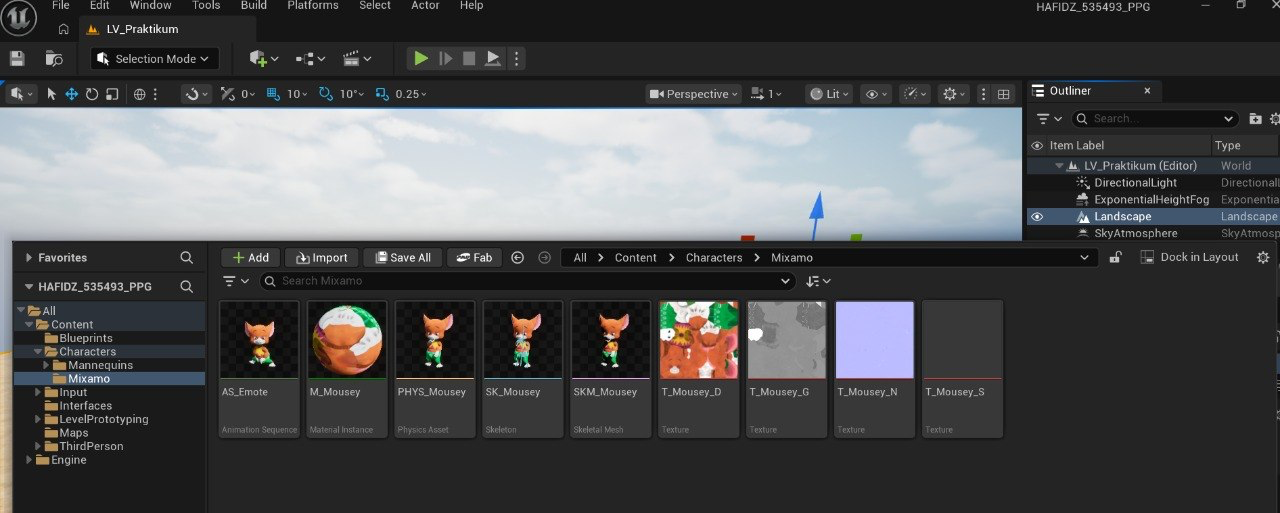
\includegraphics[width=0.9\textwidth]{images/ss-08-naming-convention-mixamo.png}}
		      \caption{Struktur aset folder Mixamo yang telah dirapikan menggunakan prefiks standar Epic Games.}
		      \label{fig:ss-naming-convention-mixamo}
	      \end{figure}

	      Pada Gambar \ref{fig:ss-naming-convention-mixamo}, panel Content Drawer menampilkan daftar aset dengan awalan prefiks yang seragam. Standardisasi nama mempermudah pencarian aset pada menu referensi Blueprint dan mencegah tertukarnya aset kerangka tulang dengan aset jala karakter.

\end{enumerate}

\subsection{Proses Retargeting dan Konfigurasi Animation Blueprint}

\begin{enumerate}
	\item \textbf{Retarget Animasi dari Mannequin ke Karakter Mixamo.} Aset animasi dasar Mannequin \texttt{MM\_idle} yang berada di folder \texttt{Characters/Mannequins/Anims/Unarmed} diklik kanan, lalu dipilih opsi \textbf{Retarget Animations}. Pada jendela retargeting, kolom \textbf{Target Skeletal Mesh} diisi dengan \textbf{SKM\_Mousey}. Setelah keselarasan gerakan kedua karakter dipastikan pada pratinjau, tombol \textbf{Export Retarget Assets} ditekan menuju folder \texttt{Content/Characters/Mixamo}.

	      \begin{figure}[H]
		      \centering
		      \customfbox{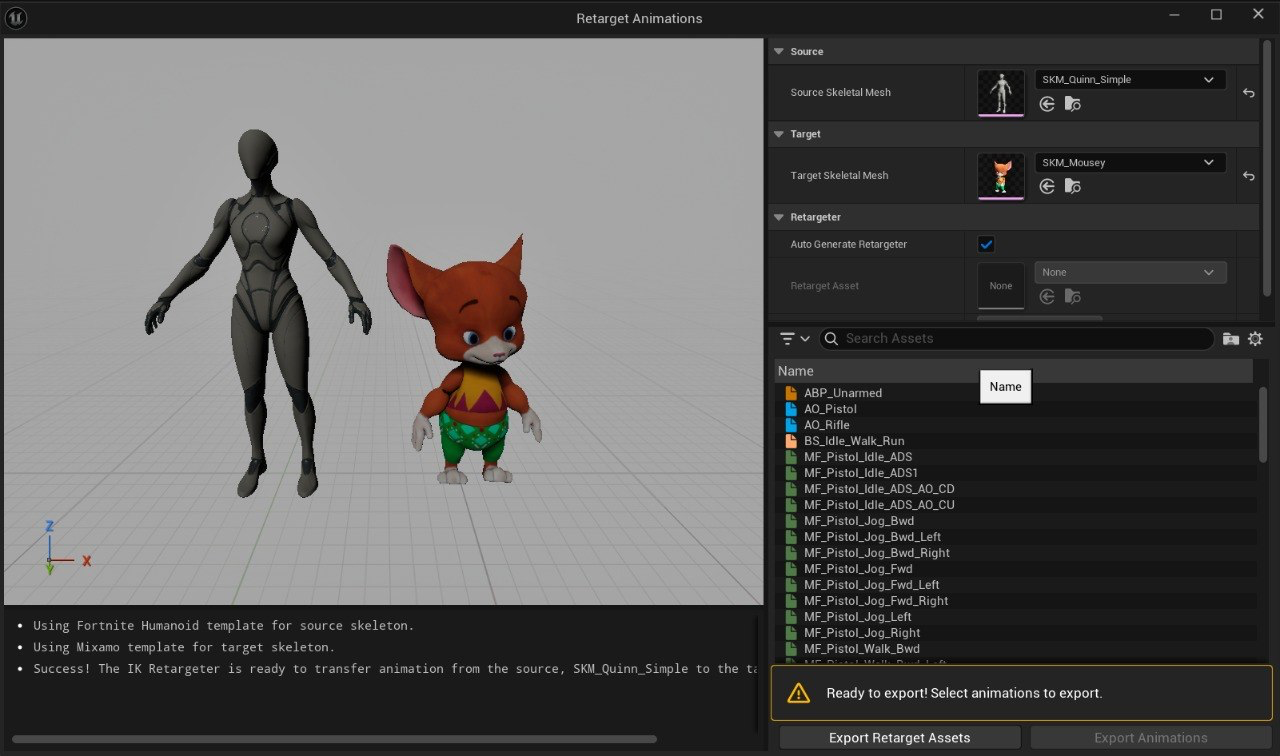
\includegraphics[width=0.9\textwidth]{images/ss-09-retarget-animations-window.png}}
		      \caption{Jendela Retarget Animations yang menampilkan komparasi gerakan Mannequin dan karakter target SKM\_Mousey.}
		      \label{fig:ss-retarget-animations-window}
	      \end{figure}

	      Gambar \ref{fig:ss-retarget-animations-window} memperlihatkan dua viewport berdampingan: karakter Mannequin sebagai sumber di sisi kiri dan karakter Mousey sebagai target di sisi kanan. Sistem IK Retargeter menerjemahkan pose A-Pose ke proporsi kerangka Mixamo secara presisi, menghasilkan aset retarget baru yang siap digunakan untuk locomotion.

	\item \textbf{Pembuatan Animation Blueprint Karakter Kustom.} Pada folder \texttt{Mixamo}, klik kanan dilakukan untuk membuat aset baru melalui menu \textbf{Animation > Animation Blueprint}. Pada jendela pemilihan kerangka target, skeleton milik karakter Mixamo, yaitu \textbf{SK\_Mousey}, dipilih sebagai acuan dasar. Berkas ini diberi nama \textbf{ABP\_Mousey}.

	      \begin{figure}[H]
		      \centering
		      \customfbox{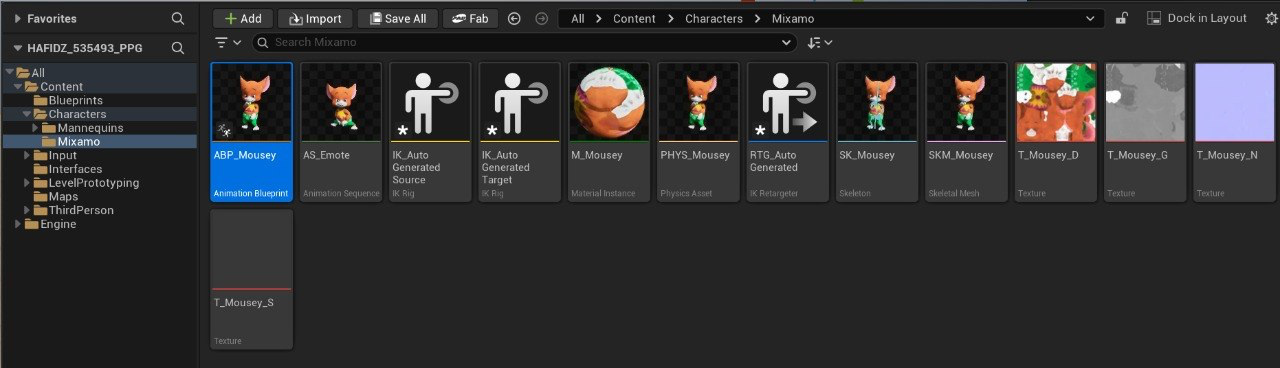
\includegraphics[width=0.9\textwidth]{images/ss-10-create-abp-mixamo.png}}
		      \caption{Pembuatan aset Animation Blueprint baru berbasis kerangka skeleton SK\_Mousey.}
		      \label{fig:ss-create-abp-mixamo}
	      \end{figure}

	      Pada Gambar \ref{fig:ss-create-abp-mixamo}, dialog pemilihan kerangka mengaitkan Animation Blueprint dengan hierarki sendi SK\_Mousey. Langkah ini krusial agar seluruh grafik pose dan pembauran gerak mengenali nama tulang yang dimiliki oleh model kustom tersebut.

	\item \textbf{Penyusunan Node Retarget Pose From Mesh pada AnimGraph.} Berkas \texttt{ABP\_Mousey} dibuka pada tab \textbf{AnimGraph}. Node baru bernama \textbf{Retarget Pose From Mesh} ditambahkan ke area grafik. Pin pose keluarannya disambungkan langsung ke pin \textbf{Result} pada node \textbf{Output Pose}. Pada panel Details node tersebut, properti \textbf{IKRetargeter Asset} dihubungkan ke aset retargeter yang dihasilkan dari proses ekspor sebelumnya.

	      \begin{figure}[H]
		      \centering
		      \customfbox{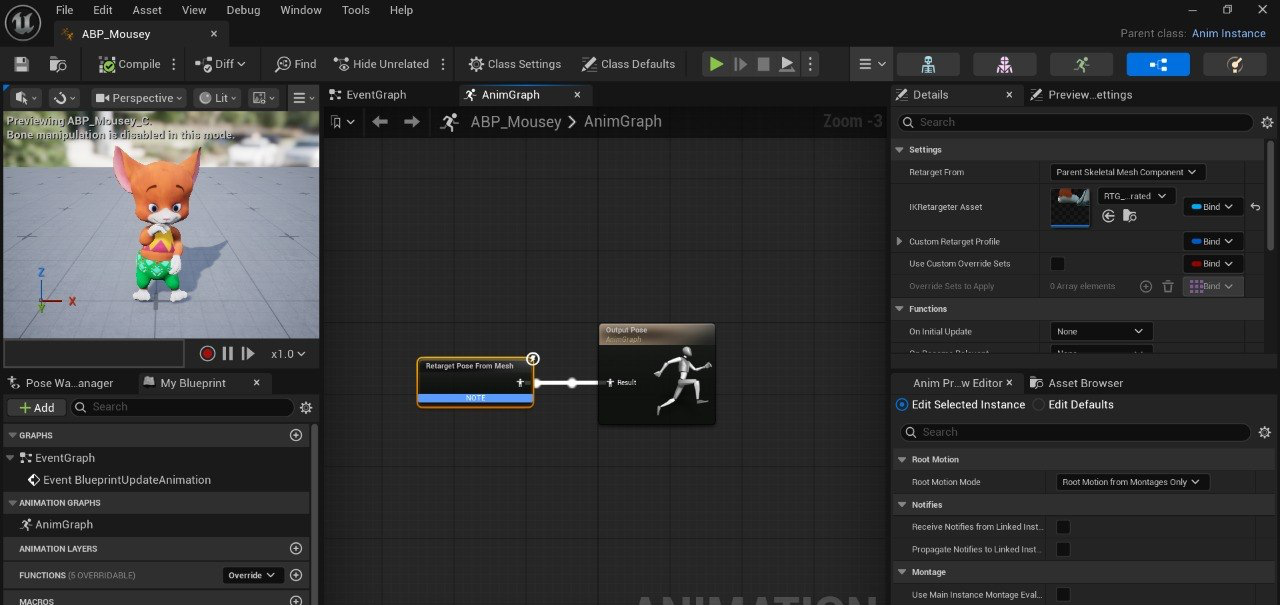
\includegraphics[width=0.9\textwidth]{images/ss-11-abp-retarget-pose-from-mesh.png}}
		      \caption{Rangkaian node Retarget Pose From Mesh yang terhubung ke Output Pose pada AnimGraph ABP\_Mousey.}
		      \label{fig:ss-abp-retarget-pose}
	      \end{figure}

	      Gambar \ref{fig:ss-abp-retarget-pose} memperlihatkan alur logika AnimGraph yang ringkas. Node Retarget Pose From Mesh bertindak sebagai penerima pose dinamis dari skeletal mesh utama Mannequin saat runtime, memetakan kembali transformasi tulang ke kerangka Mousey secara berkelanjutan.

	\item \textbf{Penerapan Mesh dan Anim Class pada Karakter Utama.} Berkas Blueprint karakter pemain \textbf{BP\_ThirdPersonCharacter} dibuka. Komponen \textbf{Mesh (CharacterMesh0)} dipilih pada panel Components. Pada panel Details, slot \textbf{Skeletal Mesh Asset} diganti menjadi \textbf{SKM\_Mousey}, dan properti \textbf{Anim Class} disetel ke \textbf{ABP\_Mousey}.
	      \begin{figure}[H]
		      \centering
		      \customfbox{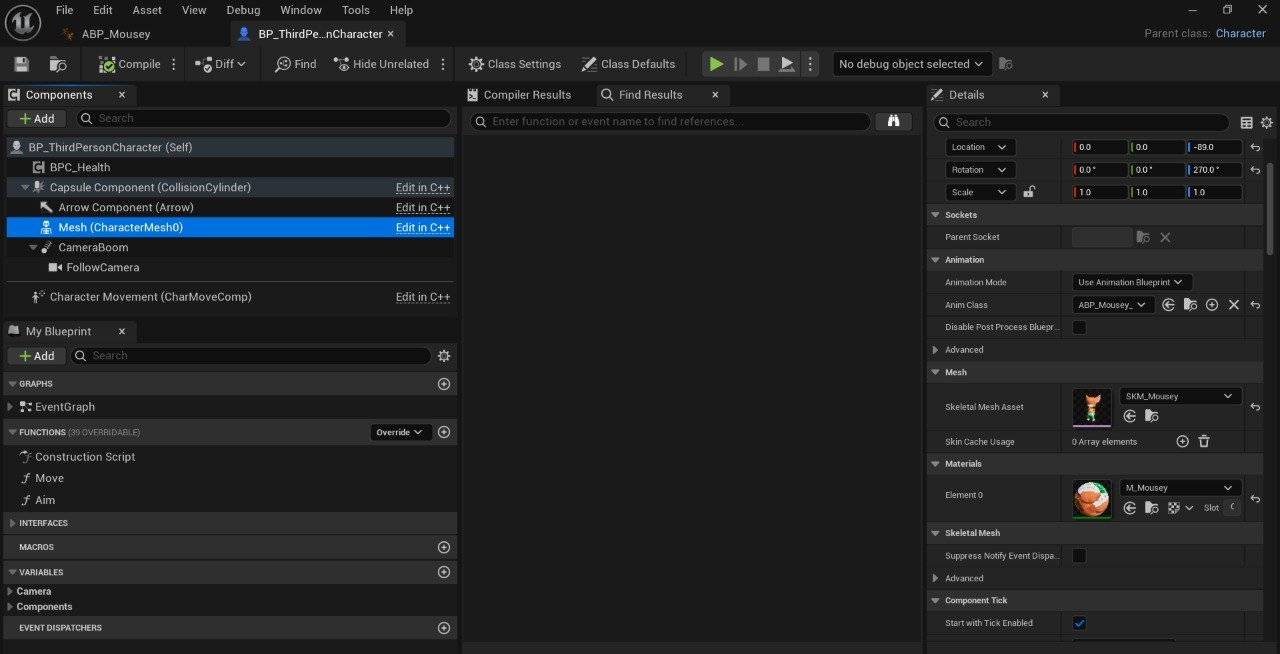
\includegraphics[width=0.9\textwidth]{images/ss-12-character-mesh-abp-setup.png}}
		      \caption{Konfigurasi Skeletal Mesh SKM\_Mousey dan Anim Class ABP\_Mousey pada BP\_ThirdPersonCharacter.}
		      \label{fig:ss-character-mesh-setup}
	      \end{figure}

	      Pada Gambar \ref{fig:ss-character-mesh-setup}, viewport editor karakter menampilkan wujud visual Mousey yang menggantikan model robot Mannequin. Pengaitan kelas animasi ABP\_Mousey memastikan karakter kustom langsung merespons perintah navigasi gerak berjalan dan melompat.

	\item \textbf{Penyembunyian Mesh Mannequin dan Optimasi Animasi.} Jika mesh Mannequin digunakan sebagai komponen induk terpisah, visibilitasnya dinonaktifkan dengan menghilangkan tanda centang pada opsi \textbf{Visible} di bagian Rendering. Selanjutnya pada seksi Optimization, properti \textbf{Visibility Based Anim Tick Option} diubah nilainya menjadi \textbf{Always Tick Pose and Refresh Bones}.

	      \begin{figure}[H]
		      \centering
		      \customfbox{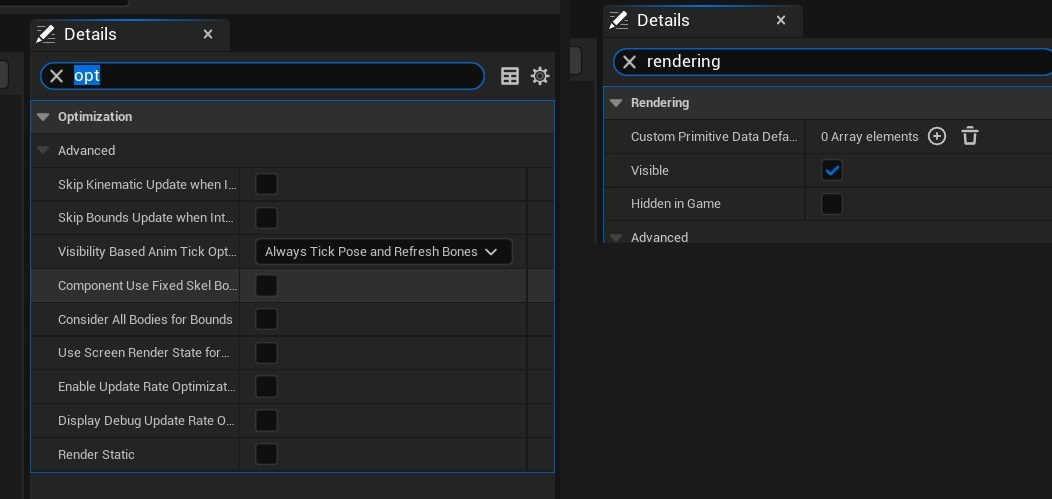
\includegraphics[width=0.9\textwidth]{images/ss-13-hide-mesh-mannequin-settings.png}}
		      \caption{Pengaturan opsi Visible dan penyetelan Always Tick Pose and Refresh Bones pada panel Details.}
		      \label{fig:ss-hide-mesh-mannequin}
	      \end{figure}

	      Gambar \ref{fig:ss-hide-mesh-mannequin} menyoroti parameter optimasi animasi. Pengaturan Always Tick Pose and Refresh Bones menjaga agar siklus evaluasi pose kerangka Mannequin tetap dihitung oleh CPU pada setiap frame meskipun wujud fisiknya tidak tampak di layar. Tanpa opsi ini, node retargeting pada karakter kustom akan kehilangan pasokan data pose gerak saat dimainkan.

\end{enumerate}

\subsection{Implementasi dan Pemicuan Animation Montage}

\begin{enumerate}
	\item \textbf{Konversi Animation Sequence Menjadi AnimMontage.} Pada folder \texttt{Mixamo}, aset rekaman animasi aksi diklik kanan. Menu konteks \textbf{Create > Create AnimMontage} dipilih untuk membungkus urutan animasi ke dalam format montage. Berkas montage baru tersebut disimpan dengan nama \textbf{AM\_Emote}.

	      \begin{figure}[H]
		      \centering
		      \customfbox{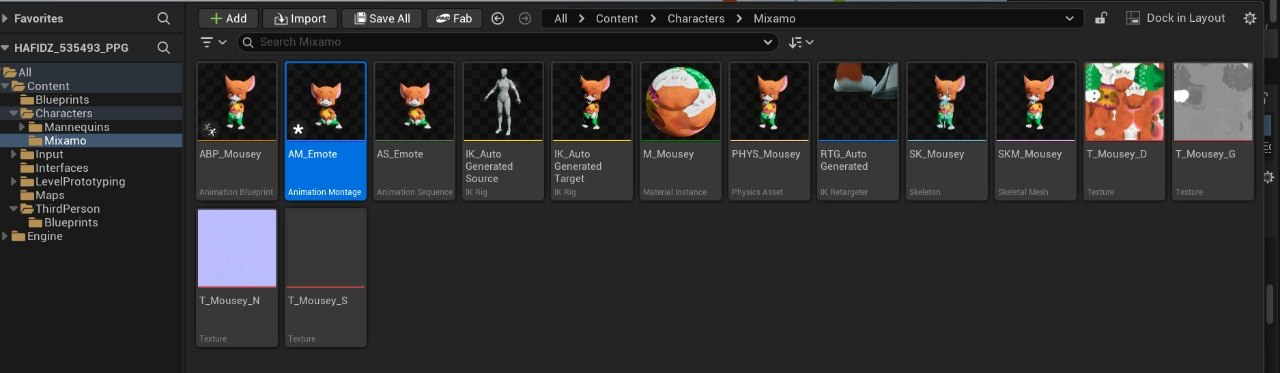
\includegraphics[width=0.9\textwidth]{images/ss-14-create-anim-montage.png}}
		      \caption{Pembuatan aset Animation Montage AM\_Emote dari Animation Sequence pada Content Drawer.}
		      \label{fig:ss-create-anim-montage}
	      \end{figure}

	      Pada Gambar \ref{fig:ss-create-anim-montage}, berkas AM\_Emote terbentuk dengan ikon strip film khas montage. Struktur montage memungkinkan animasi aksi ini disisipkan di atas animasi gerak dasar pemain tanpa merombak state machine pada grafik animasi utama.

	\item \textbf{Penyisipan Node Slot DefaultSlot pada AnimGraph.} Berkas \texttt{ABP\_Mousey} dibuka kembali pada tab \textbf{AnimGraph}. Node baru \textbf{Slot 'DefaultSlot'} disisipkan di antara node \textit{Retarget Pose From Mesh} dan node \textit{Output Pose}. Pin keluaran pose dari node retarget dihubungkan ke pin masukan \textit{Source} pada Slot DefaultSlot, lalu keluarannya diteruskan ke Output Pose.

	      \begin{figure}[H]
		      \centering
		      \customfbox{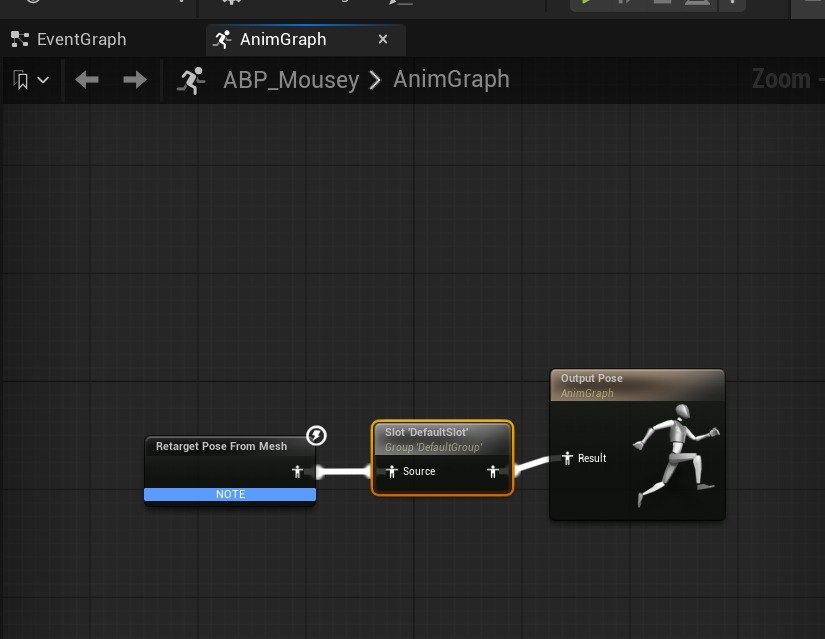
\includegraphics[width=0.9\textwidth]{images/ss-15-abp-default-slot.png}}
		      \caption{Penambahan node Slot DefaultSlot pada AnimGraph ABP\_Mousey untuk menerima pemutaran montage.}
		      \label{fig:ss-abp-default-slot}
	      \end{figure}

	      Gambar \ref{fig:ss-abp-default-slot} menampilkan susunan grafik animasi yang telah dilengkapi slot pembauran. Node Slot DefaultSlot bertindak sebagai pintu masuk lapisan animasi luar. Ketika sebuah montage dipanggil, data pose dari slot ini akan menimpa pose dasar secara temporer sesuai kurva transisi pembauran.

	\item \textbf{Penyusunan Logika Pemicu Input pada Event Graph.} Editor \texttt{BP\_ThirdPersonCharacter} dibuka pada tab \textbf{Event Graph}. Node masukan \textbf{Keyboard Event E} ditambahkan ke kanvas logika. Pin eksekusi \textbf{Pressed} ditarik dan dihubungkan ke node fungsi \textbf{Play Anim Montage}. Pada parameter node fungsi tersebut, slot \textbf{Anim Montage} diisi dengan aset \textbf{AM\_Emote}.

	      \begin{figure}[H]
		      \centering
		      \customfbox{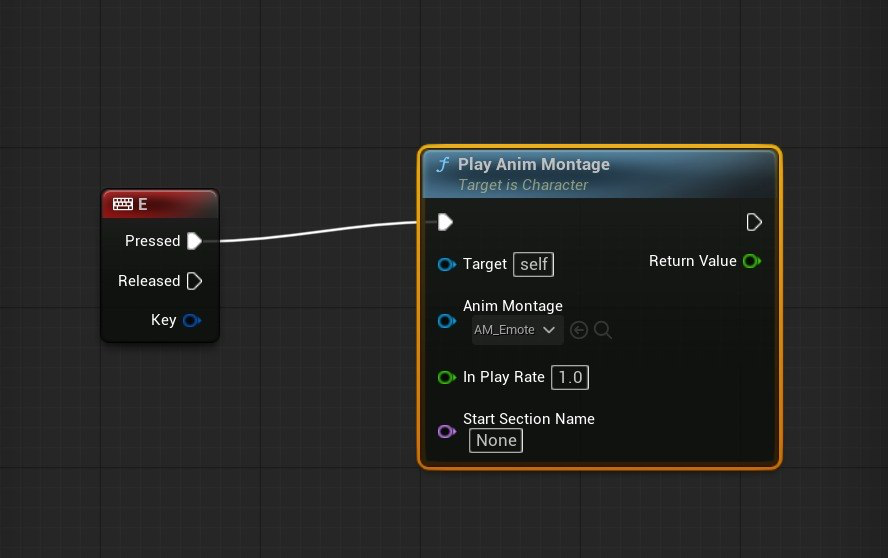
\includegraphics[width=0.9\textwidth]{images/ss-16-event-graph-play-montage.png}}
		      \caption{Rangkaian Event Graph BP\_ThirdPersonCharacter yang memicu node Play Anim Montage saat tombol E ditekan.}
		      \label{fig:ss-event-graph-play-montage}
	      \end{figure}

	      Pada Gambar \ref{fig:ss-event-graph-play-montage}, sambungan kabel putih eksekusi menghubungkan event penekanan tombol E dengan instruksi pemutaran montage. Blueprint dikompilasi dan disimpan tanpa memunculkan pesan peringatan atau galat logika.

\end{enumerate}

\section{Hasil Akhir}
Pengujian integrasi sistem dilakukan langsung di dalam editor Unreal Engine 5.8 dengan membuka level \textbf{LV\_Praktikum} dan menekan tombol \textbf{Play}. Karakter kustom Mousey berhasil muncul di atas bentang alam berkontur yang diterangi oleh tata cahaya atmosferik realistis. Seluruh input navigasi dasar (gerakan maju, mundur, menyamping, dan melompat) dieksekusi dengan mulus berkat data retargeting yang mengalir dari sistem pergerakan Mannequin.

\begin{figure}[H]
	\centering
	\customfbox{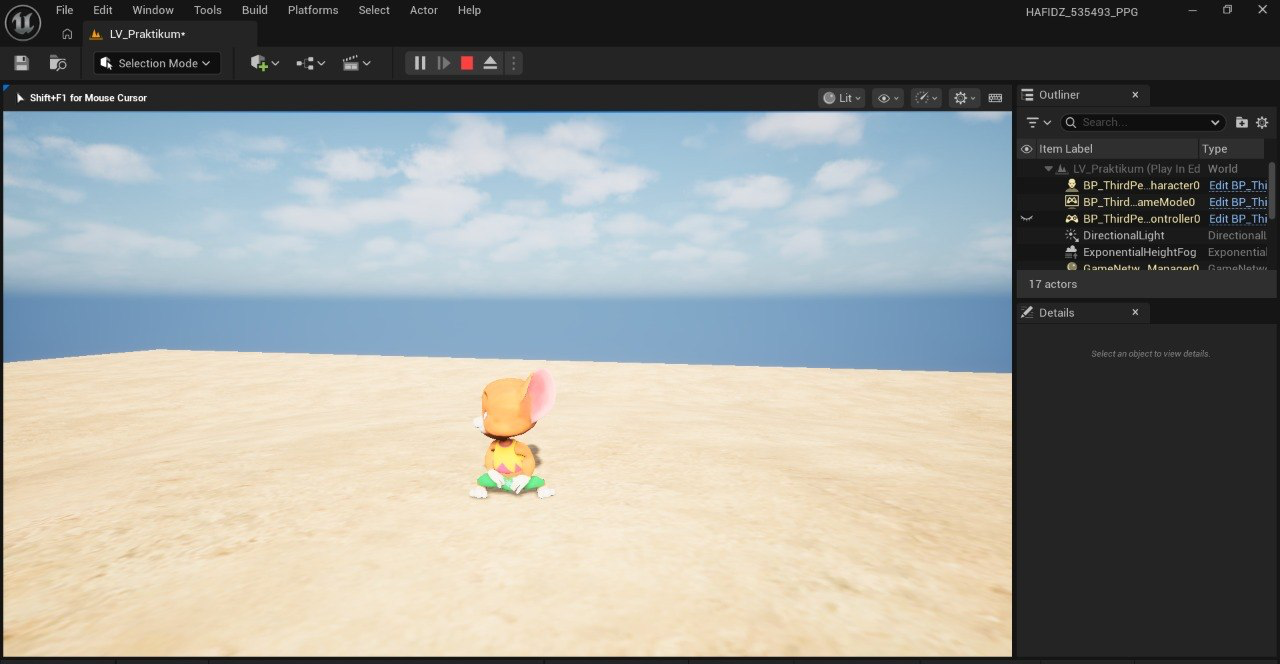
\includegraphics[width=0.95\textwidth]{images/ss-17-hasil-akhir-montage-gameplay.png}}
	\caption{Pengujian gameplay di level LV\_Praktikum: karakter kustom Mixamo memainkan animasi montage di atas bentang alam saat tombol E ditekan.}
	\label{fig:hasil-akhir-gameplay}
\end{figure}

Saat karakter sedang berdiri maupun berjalan di atas permukaan berkontur, penekanan tombol \textbf{E} pada keyboard langsung memicu node \texttt{Play Anim Montage}. Karakter mengeksekusi gerakan aksi tarian emote secara utuh dengan transisi pembauran yang halus. Setelah durasi pemutaran animasi montage selesai, kontrol karakter secara otomatis kembali ke pose navigasi normal tanpa mengalami sentakan visual (\textit{glitch}). Hasil pengujian pada Gambar \ref{fig:hasil-akhir-gameplay} membuktikan bahwa bentang alam, tata cahaya lingkungan, alur retargeting kerangka Mixamo, serta sistem slot Animation Montage telah terintegrasi secara fungsional sesuai ketentuan modul praktikum.

\clearpage

\chapter{Kesimpulan}
Praktikum Pertemuan 6 memberikan pemahaman terpadu mengenai konstruksi lingkungan bentang alam, tata cahaya atmosferik, sistem kerangka digital, serta kontrol animasi karakter pada Unreal Engine 5.8. Pemilihan template \textit{Empty Level} terbukti menjadi pendekatan yang tepat untuk prototipe berukuran sedang karena menghasilkan objek \texttt{Landscape} murni, terhindar dari kerumitan partisi data instansiasi pada sistem World Partition. Pemanfaatan jendela \textit{Environment Light Mixer} mempercepat penataan atmosfer realistis dengan menyatukan kendali lima komponen pencahayaan lingkungan secara instan.

Perbedaan pose dasar antara kerangka Mixamo (T-Pose) dan Unreal Engine Mannequin (A-Pose) berhasil dijembatani melalui mekanisme \textit{IK Retargeting}. Penerapan node \texttt{Retarget Pose From Mesh} pada Animation Blueprint memungkinkan model kustom memanfaatkan pustaka logika locomotion yang telah ada tanpa perlu merekam ulang pose gerak dari awal. Kunci kelancaran alur kerja ini terletak pada aktivasi opsi \textit{Always Tick Pose and Refresh Bones}, yang menjaga pembaruan transformasi tulang di latar belakang saat mesh sumber disembunyikan.

Penggunaan \textit{Animation Montage} melengkapi kendali karakter melalui sistem slot modular. Penambahan node \texttt{Slot 'DefaultSlot'} pada AnimGraph serta integrasi pemanggilan node fungsi \texttt{Play Anim Montage} melalui tombol keyboard E berhasil mengeksekusi animasi aksi sesaat secara mulus. Karakter mampu beralih dari gerakan berjalan ke aksi ekspresi tanpa merusak alur state machine utama, membuktikan seluruh target pembelajaran praktikum telah tercapai dengan baik.

\clearpage
\addcontentsline{toc}{chapter}{Daftar Pustaka}
\renewcommand{\bibname}{Daftar Pustaka}
\begin{spacing}{1.05}
	\begin{thebibliography}{99}
		\setlength{\itemsep}{0.15em}
		\bibitem{modul6} Tim Dosen Praktikum Pengembangan Game, ``Modul Praktikum Pengembangan Game Pertemuan 6: Landscape, Rig, Retarget, dan Animation'', Departemen Teknik Elektro dan Informatika, Sekolah Vokasi, Universitas Gadjah Mada, Yogyakarta, 2026.
		\bibitem{epic-levels} Epic Games, ``Working with Levels in Unreal Engine'', Unreal Engine 5.8 Documentation, 2026. [Daring]. Tersedia: \url{https://dev.epicgames.com/documentation/en-us/unreal-engine/working-with-levels-in-unreal-engine}.
		\bibitem{epic-lightmixer} Epic Games, ``Environmental Light Mixer in Unreal Engine'', Unreal Engine 5.8 Documentation, 2026. [Daring]. Tersedia: \url{https://dev.epicgames.com/documentation/en-us/unreal-engine/environmental-light-mixer-in-unreal-engine}.
		\bibitem{epic-landscape} Epic Games, ``Creating Landscapes in Unreal Engine'', Unreal Engine 5.8 Documentation, 2026. [Daring]. Tersedia: \url{https://dev.epicgames.com/documentation/en-us/unreal-engine/creating-landscapes-in-unreal-engine}.
		\bibitem{epic-sculpt} Epic Games, ``Sculpt Mode in Unreal Engine'', Unreal Engine 5.8 Documentation, 2026. [Daring]. Tersedia: \url{https://dev.epicgames.com/documentation/en-us/unreal-engine/sculpt-mode-in-unreal-engine}.
		\bibitem{epic-skeletal} Epic Games, ``Skeletal Mesh Animation System in Unreal Engine'', Unreal Engine 5.8 Documentation, 2026. [Daring]. Tersedia: \url{https://dev.epicgames.com/documentation/en-us/unreal-engine/skeletal-mesh-animation-system-in-unreal-engine}.
		\bibitem{epic-retargeter} Epic Games, ``IK Rig and IK Retargeter in Unreal Engine'', Unreal Engine 5.8 Documentation, 2026. [Daring]. Tersedia: \url{https://dev.epicgames.com/documentation/en-us/unreal-engine/ik-rig-animation-retargeting-in-unreal-engine}.
		\bibitem{epic-montage} Epic Games, ``Animation Montage in Unreal Engine'', Unreal Engine 5.8 Documentation, 2026. [Daring]. Tersedia: \url{https://dev.epicgames.com/documentation/en-us/unreal-engine/animation-montage-in-unreal-engine}.
		\bibitem{epic-naming} Epic Games, ``Recommended Asset Naming Conventions in Unreal Engine Projects'', Unreal Engine 5.8 Documentation, 2026. [Daring]. Tersedia: \url{https://dev.epicgames.com/documentation/en-us/unreal-engine/recommended-asset-naming-conventions-in-unreal-engine-projects}.
		\bibitem{mixamo-web} Adobe Systems, ``Mixamo: 3D Characters and Animations for Games and Film'', 2026. [Daring]. Tersedia: \url{https://www.mixamo.com/}.
		\bibitem{epic-metahuman} Epic Games, ``MetaHuman Documentation'', Unreal Engine Documentation, 2026. [Daring]. Tersedia: \url{https://dev.epicgames.com/documentation/en-us/metahuman}.
	\end{thebibliography}
\end{spacing}

\end{document}
